\chapter{Определение и свойства функции}

\section{Определения}

\mcdfn{Определение функции}{
    Множество пар $\{ (x, y) \in \Rset[2] | x \in D_f \wedge y \in E_f \} $ называется 
    функцией $f$ с областью определения $D_f$ и областью значения $E_f$, если 
    $ \forall x \in D_f \, \exists! y \in E_f: (x, y) \in f $ (для удобства  $ (x, y) \in f $ обозначают как $ f(x) = y $)

    Обозначение функции: $ f: X \to Y $

    В данном обозначении подразумевают, что $ D_f = X, E_f \subseteq Y $
}

\mcex{}{
    $ f: \mathbb{N} \cup \{ 0 \} \to \Rset $

    $ \forall n \in \mathbb{N} \cup \{ 0 \}: f(n) = (-1)^{n + 1} \cdot \left\lceil \frac{n}{2} \right\rceil $, 
    в данном случае $ D_f = \mathbb{N} \cup \{ 0 \}, E_f = \mathbb{Z} \subset \Rset $

    Т.к. несложно установить, что $E_f = \mathbb{Z}$, то можно написать $ f: \mathbb{N} \cup \{ 0 \} \to \mathbb{Z} $
}

\mcdfn{Определение инъективной функции}{
    Функция $f$ называется инъективной, если $ \forall y \in E_f \, \exists! x \in D_f: f(x) = y $

    Это эквивалентно тому, что $ \forall x_1, x_2 \in D_f: (x_1 \ne x_2 \implies f(x_1) \ne f(x_2)) $

    (говорят, что $f$ - инъекция)
}

\mcex{} {
    $ \forall n \in \mathbb{N} $ функция $f(x) = x^{2 n - 1}$ является инъективной

    $ \forall n \in \mathbb{N} $ функция $f(x) = x^{2 n}$ не является инъективной
}

\mcdfn{Определение сюръективной функции}{
    Функция $f: X \to Y$ называется сюръективной для множества $Y$, если $ E_f = Y $

    (говорят, что $f$ - сюръекция)
    
    Когда говорят, что $f$ сюръективна, не уточняя множество, то подразумевают, что $f$ сюръективна для $Y$

}

\mcex{}{
    Функция $\sin: \Rset \to \Rset $ не сюръективна для $\Rset$, но сюръективна для $[-1; 1]$
}

\mcdfn{Определение биективной функции}{
    Функция $f: X \to Y$ называется биективной, если она инъективна и сюръективна

    (говорят, что $f$ - биекция)
}

\mcex{}{
    Функция $ f: \mathbb{N} \cup \{ 0 \} \to \mathbb{Z} $, такая что \\
    $ \forall n \in \mathbb{N} \cup \{ 0 \}: f(n) = (-1)^{n + 1} \cdot \left\lceil \frac{n}{2} \right\rceil $
    - биекция между $\mathbb{N} \cup \{ 0 \}$ и $\mathbb{Z}$

    (как следствие, показали, что $\mathbb{N} \cup \{ 0 \} \sim \mathbb{Z}$, т.е. множества равномощны)
}

\section{Пределы}

\subsection{Определение предела функции по Коши}

\mcdfn{Определение предела функции по Коши}
{
    \[
    \lim_{x \to x_0} f(x) = A \iff
    \forall \veps > 0 \,
    \exists \delta = \delta(\veps) \,
    \forall x \in \dot{U}_\delta(x_0):
    f(x) \in U_\veps(A) \]
}

\nt
{
    При этом
    $ \dot{U}_\delta(+\infty) = (\delta; +\infty) $,
    $ \dot{U}_\delta(-\infty) = (-\infty; \delta) $,
    $ \dot{U}_\delta(\infty) = (-\infty; \delta) \cup (\delta; +\infty) $
}

\subsection{Определение предела функции по Гейне}

\mcdfn{Определение предела функции по Гейне}
{
    \[
    \lim_{x \to x_0} f(x) = A \iff
    \forall \NumSeq{x_n}:
    (x_n \ne x_0 \wedge \lim_{n \to +\infty} x_n = x_0 \implies \lim_{n \to +\infty} f(x_n) = A)\]
}

\subsection{Теорема об эквивалентности определений по Коши и по Гейне}

\mcthm{Теорема об эквивалентности определений по Коши и по Гейне}{
    Определение предела функции по Коши эквивалентно определению предела функции по Гейне

\mcprf{
\begin{split}
    & "\implies" \\
    & \text{Распишем определение по Коши: }
        \forall \xi > 0 \, \exists \delta = \delta(\xi) > 0 \, \forall x \in \dot{U}_\delta(x_0): | f(x) - A | < \xi \,\,\, (1) \\
    & \text{Пусть дана ч.п., удовлетворяющая условиям посылки импликации, т.е. } \\
    & \NumSeq{x_n}: x_n \underset{n \to +\infty}{\to} x_0 \wedge \forall n \in \Nset: x_n \ne x_0 \\
    & \text{По определению это означает, что } \\
    & \forall \lambda > 0 \, \exists N(\lambda) \in \Nset[] \, \forall n > N(\lambda): 0 < | x_n - x_0 | < \lambda \,\,\, (2) \\ 
    & \text{Хотим доказать: } \\
    & \forall \veps > 0 \, \exists N_1(\veps) \in \Nset[] \, \forall n > N_1(\veps): | f(x_n) - A | < \veps \\
    & \text{Пусть дано $\veps > 0$, тогда по (2):} \\ 
    & \forall n > N(\delta(\veps)): 0 < | x_n - x_0 | < \delta(\veps) \\
    & \text{Это равносильно тому, что } \forall n > N(\delta(\veps)): x_n \in \dot{U}_{\delta(\veps)}(x_0) \\
    & \text{Тогда по (1) получим: } \forall n > N(\delta(\veps)): | f(x) - A | < \veps \\
    & \text{Т.е. мы доказали искомое высказывание, положив } N_1(\veps) := N(\delta(\veps)) \\
    & "\impliedby" \\
    & \text{Предположим от противного, т.е. выполнено определение по Гейне, но по Коши не выполнено:} \\
    & \forall \NumSeq{x_n}: x_n \underset{n \to +\infty}{\to} x_0 \wedge \forall n \in \Nset: x_n \ne x_0 \implies f(x_n) \underset{n \to +\infty}{\to} A \,\,\, (3) \\
    & \exists \veps_0 > 0 \, \forall \delta > 0 \, \exists x \in \dot{U}_\delta(x_0): | f(x) - A | \ge \veps_0 \,\,\, (4) \\
    & \text{Для любого $n \in \Nset$ рассмотрим $\delta_n = \frac{1}{n}$ и $x \in \dot{U}_{\delta_n}(x_0)$ из (4) обозначим как $x_n$}  \\
    & \text{Тогда по (4): } \forall n \in \Nset[]: | f(x_n) - A | \ge \veps_0 \\
    & \forall n \in \Nset[]: 
        x_0 - \frac{1}{n} < x_n < x_0 + \frac{1}{n} 
        \implies x_n \underset{n \to +\infty}{\to} x_0 
        \text{ по теореме о пределе зажатой последовательности} \\
    & \text{Получили ч.п., такую что } 
        x_n \underset{n \to +\infty}{\to} x_0 
        \wedge \forall n \in \Nset[]: x_n \ne x_0 \\
    & \text{Тогда по определению сходимости по Гейне (3): } f(x_n) \underset{n \to +\infty}{\to} A \implies \\
    & \implies \exists N(\veps_0) \, \forall n > N(\veps_0): | f(x_n) - A | < \veps_0 \implies \Contradiction \\
\end{split}
}
}

\subsection{Определение одностороннего предела функции}

\mcdfn{Односторонний предел функции}
{
    Левосторонним пределом функции называют предел функции по Коши $ f $ при $ x \to x_0 $ слева, то есть

    \[
    \lim_{x \to x_0-} f(x) = A \iff
    \forall \veps > 0
    \exists \delta = \delta(\veps)   
    \forall x \in (x_0 - \delta; x_0):
    f(x) \in U_\veps(A) \]

    Правосторонним пределом функции называют предел функции по Коши $ f $ при $ x \to x_0 $ справа, то есть

    \[
    \lim_{x \to x_0+} f(x) = A \iff
    \forall \veps > 0
    \exists \delta = \delta(\veps)   
    \forall x \in (x_0; x_0 + \delta):
    f(x) \in U_\veps(A) \]
}

\subsection{Свойство предела функции}

\mcthm{Свойство предела функции при $ x \to x_0, x_0 \in \Rset $}
{
    \[ \lim_{x \to x_0} f(x) = A \iff \lim_{x \to x_0+} f(x) = \lim_{x \to x_0-} f(x) = A \text{, где } A \in \ExtRset \]

\mcprf{
\begin{split}
    & "\implies" \\
    & \text{Дано:}
        \forall \veps > 0 \,
            \exists \delta = \delta(\veps) > 0 \,
            \forall x \in \dot{U}_\delta(x_0): \,
            f(x) \in U_\veps(A) \\
    & \text{Тогда:} \\
    & \forall \veps > 0 \,
        \exists \delta = \delta(\veps) > 0 \,
        \forall x \in (x_0; x_0 + \delta): \,
        f(x) \in U_\veps(A) \\
    & \forall \veps > 0 \,
        \exists \delta = \delta(\veps) > 0 \,
        \forall x \in (x_0 - \delta; x_0): \,
        f(x) \in U_\veps(A) \\
    & "\impliedby" \\
    & \text{Дано:} \\
    & \forall \veps > 0 \,
        \exists \delta_1 = \delta_1(\veps) > 0 \,
        \forall x \in (x_0; x_0 + \delta_1): \,
        f(x) \in U_\veps(A) \\
    & \forall \veps > 0 \,
        \exists \delta_2 = \delta_2(\veps) > 0 \,
        \forall x \in (x_0 - \delta_2; x_0): \,
        f(x) \in U_\veps(A) \\
    & \text{Положим } \delta(\veps) = \min(\delta_1(\veps), \delta_2(\veps)) \text{, тогда:} \\
    & \forall \veps > 0 \,
        \exists \delta = \delta(\veps) > 0 \,
            \forall x \in \dot{U}_\delta(x_0) \subseteq (x_0 - \delta_2; x_0) \cup (x_0; x_0 + \delta_1): \,
            f(x) \in U_\veps(A) \\
\end{split}
}
}

\subsection{Бесконечные пределы}

\mcdfn{Бесконечные пределы}
{
    
\begin{tabular}{rl}
    & $\bullet$
        $ \lim_{x \to x_0} f(x) = +\infty \iff
        \forall M > 0 \, \exists \delta(M) > 0 \, \forall x \in \dot{U}_{\delta}(x_0): f(x) > M $ \\
    & $\bullet$
        $ \lim_{x \to x_0} f(x) = -\infty \iff
        \forall M > 0 \, \exists \delta(M) > 0 \, \forall x \in \dot{U}_{\delta}(x_0): f(x) < -M $ \\
    & $\bullet$
        $ \lim_{x \to x_0} f(x) = \infty \iff
        \forall M > 0 \, \exists \delta(M) > 0 \, \forall x \in \dot{U}_{\delta}(x_0): | f(x) | > M $ \\
\end{tabular}
}

\mcdfn{Бесконечно малая функция}
{
    Функция называется б.м. при $x \to x_0$, если $\lim_{x \to x_0} f(x) = 0$, при этом $ x_0 \in \Rset $

    Функция называется б.м. при $x \to +\infty$, если $\lim_{x \to +\infty} f(x) = 0$

    Функция называется б.м. при $x \to -\infty$, если $\lim_{x \to -\infty} f(x) = 0$
}

\mcdfn{Бесконечно большая функция}
{
    Функция называется б.б. при $x \to x_0$, если $\lim_{x \to x_0} f(x) = \infty $, при этом $ x_0 \in \Rset $

    Функция называется б.б. при $x \to +\infty$, если $\lim_{x \to +\infty} f(x) = \infty $

    Функция называется б.б. при $x \to -\infty$, если $\lim_{x \to -\infty} f(x) = \infty $
}

\mcdfn{Ограниченная функция}
{
    Функция называется ограниченной при $x \to x_0$, если $\exists \delta > 0 \, \exists C > 0 \, \forall x \in \dot{U}_\delta(x_0): | f(x) | < C $
}

\mcdfn{Отделимая от нуля функция}
{
    Функция называется отделимой от нуля при $x \to x_0$, если 
    $\exists \delta > 0 \, \exists \veps_0 > 0 \, \forall x \in \dot{U}_\delta(x_0): | f(x) | > \veps_0 $ 
}


\nt{
    Связь функций при $ x \to x_0 $, где $ x $ - аргумент обоих функций, 
    $ x_0 $ - число, к которому стремится аргумент обоих функций:

\begin{tabular}{rl}

    & $\bullet$ $ \frac{1}{\text{б.б.}} = \text{б.м.} $ \\
    & $\bullet$ $ \frac{1}{\text{б.м.}} = \text{б.б.} $ \\
    & $\bullet$ $ \frac{1}{\text{ограниченная}} = \text{отделимая от нуля} $ \\
    & $\bullet$ $ \frac{1}{\text{отделимая от нуля}} = \text{ограниченная} $ \\
\end{tabular}
}

\section{Теорема о зажатой функции}

\mcthm{Теорема о зажатой функции}
{
\begin{minipage}[t]{\textwidth}
$$
\left. \begin{tabular}{l}
    $ f(x): \Rset \to \Rset, g(x): \Rset \to \Rset, h(x): \Rset \to \Rset $ \\
    $ \lim_{x \to x_0} f(x) = A $ \\
    $ \lim_{x \to x_0} h(x) = A $ \\
    $ \exists \delta > 0 \, \forall x \in \dot{U}_\delta(x_0): f(x) \le g(x) \le h(x) $
\end{tabular} \right\}
\begin{tabular}{l}
    $ \lim_{x \to x_0} g(x) = A $
\end{tabular}
$$
\end{minipage}
}

\section{Первый и второй замечательные пределы}

\mcdfn{Первый замечательный предел}
{
    \[ \lim_{x \to 0} \frac{\sin x}{x} = 1 \]

\mcprf{
\begin{split}
    & \text{Докажем неравенство $ x < \sin x < \tan x $ при 
        $ x \in \left(0; \frac{\pi}{2}\right) $} \\
    & \text{Рассмотрим единичную окружность с центром в (0; 0):} \\
    & 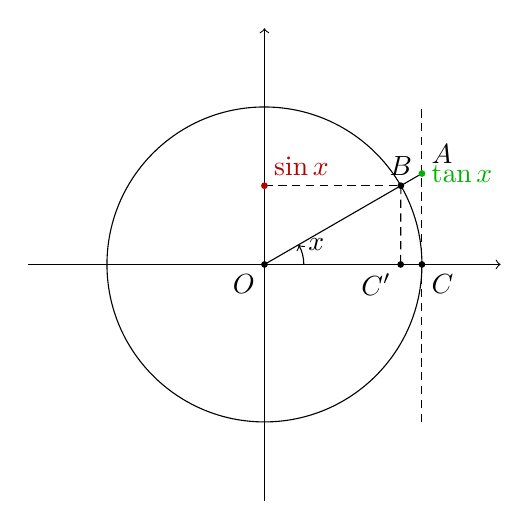
\begin{tikzpicture}
        \draw[black] (0, -0) circle (2);
        \draw[->] (-3, 0) -- (3, 0);
        \draw[->] (0, -3) -- (0, 3);
        \coordinate (A_pnt) at (30:2.31);
        \coordinate (B_pnt) at (30:2);
        \coordinate (C_p_pnt) at (1.73, 0);
        \coordinate (C_pnt) at (2, 0);
        \draw (0, 0) -- (A_pnt);
        \draw[densely dashed] (2, -2) -- (2, 2);
        \draw[densely dashed] (0, 1) -- (B_pnt);
        \filldraw[green!70!black] (A_pnt) circle(1pt) node[anchor=west]{$\tan x$};
        \filldraw[red!70!black] (0, 1) circle(1pt) node[anchor=south west]{$\sin x$};
        \draw[densely dashed] (B_pnt) -- (C_p_pnt);
        \filldraw[black] (0, 0) circle(1pt) node[anchor = north east]{$O$};
        \filldraw[black] (A_pnt) node[anchor = south west]{$A$};
        \filldraw[black] (B_pnt) circle(1pt) node[anchor = south]{$B$};
        \filldraw[black] (C_pnt) circle(1pt) node[anchor = north west]{$C$};
        \filldraw[black] (C_p_pnt) circle(1pt) node[anchor = north east]{$C'$};
        \draw[->] (0.5,0) arc (0:30:0.5) node[anchor=west]{$x$};
    \end{tikzpicture} \\
    & AC = \tan x, BC' = \sin x, \text{ дуга } \breve{BC} = x \cdot OC  \\
    & \text{Пусть $S_{BOC}, S_{AOC}$ - 
        площади соответствующих треугольников,
        $S_{\breve{BOC}}$ - площаль сектора, тогда} \\
    & S_{BOC} < S_{\breve{BOC}} < S_{AOC} \\
    & \frac{BC' OC}{2} < \frac{x OC^2}{2} < \frac{AC OC}{2} \\
    & \sin x < x < \tan x \\
    & \frac{\sin x}{x} < 1 < \frac{\sin x}{x \cos x} \\
    & \cos x < \frac{\sin x}{x} < 1 \\
    & \text{При } x \in \left(-\frac{\pi}{2}; 0\right) \text{ воспользуемся нечётностью синуса и чётностью косинуса:}\\
    & \frac{\sin x}{x} = \frac{\sin(-x)}{-x} \in (\cos(x); 1) \\
    & \text{Тогда } \forall x \in \dot{U}_{\frac{\pi}{2}}(0): \cos x < \frac{\sin x}{x} < 1 \\
    & \text{Распишем предел по определению сходимости по Коши:} 
        \forall \veps > 0 \, 
        \exists \delta(\veps) > 0 \, 
        \forall x \in \dot{U}_{\delta(\veps)}(0): 
        \left| \frac{\sin x}{x} - 1 \right| < \veps \\
    & \text{Будем выбирать только значения $\delta(\veps) \le \frac{\pi}{2}$, тогда} \\
    & \left| \frac{\sin x}{x} - 1 \right| < \veps
        \impliedby 1 - \frac{\sin x}{x} < \veps
        \impliedby 1 - \cos x < \veps
        \impliedby 1 - \cos^2 x < \veps
        \impliedby \sin^2 x < \veps \\
    &   \impliedby \sin x < \veps
        \impliedby x < \veps \\
    & \text{Показали, что если } 
        \forall \veps > 0: 
        \delta(\veps) := \min\left(\veps; \frac{\pi}{2}\right) 
        \text{, то определение предела по Коши выполняется}\\
\end{split}
}
}

\mcdfn{Второй замечательный предел}
{
    \[ \lim_{x \to +\infty} \left(1 + \frac{1}{x}\right)^x = e \]

\mcprf{
\begin{split}
    & \text{1. По определению числа Эйлера: } \lim_{n \to +\infty} \left(1 + \frac{1}{n}\right)^{n} = e \\
    & \text{По арифметике предела ч.п.: } \\
    & \lim_{n \to +\infty} \left(1 + \frac{1}{n + 1}\right)^{n} = e \\
    & \lim_{n \to +\infty} \left(1 + \frac{1}{n}\right)^{n + 1} = e \\
    & \text{По определению предела ч.п. это означает:} \\
    & \forall \veps > 0 \,
        \exists N_1(\veps) \in \Nset[] \, 
        \forall n > N_1(\veps): 
        \left| \left(1 + \frac{1}{n + 1}\right)^{n} - e \right| < \veps \\
    & \text{Последнее выражение равносильно: } e - \veps < \left(1 + \frac{1}{n + 1}\right)^{n} < e + \veps \\
    & \text{Аналогично } \\
    & \forall \veps > 0 \,
        \exists N_2(\veps) \in \Nset[] \, 
        \forall n > N_2(\veps): 
        e - \veps < \left(1 + \frac{1}{n}\right)^{n + 1} < e + \veps \\
    & \text{2. Хотим доказать: } \lim_{x \to +\infty} \left(1 + \frac{1}{x}\right)^x = e \\
    & \text{Распишем определение предела функции по Коши при $x \to +\infty$:} \\
    & \forall \veps > 0 \,
        \exists \delta = \delta(\veps) > 0 \,
        \forall x \in (\delta; +\infty):
        \left| \left(1 + \frac{1}{x}\right)^{x} - e \right| < \veps \\
    & \text{Будем рассматривать только $\delta \ge 1$, тогда:} \\
    & \forall x \in (\delta; +\infty) \,
        \exists n \in \Nset[]: n < x \le n + 1 \\
    & \text{Тогда } \left(1 + \frac{1}{n + 1}\right)^{n} < \left(1 + \frac{1}{x}\right)^{x} < \left(1 + \frac{1}{n}\right)^{n + 1} \\
    & \text{Положим } \delta(\veps) := \max\{N_1(\veps), N_2(\veps)\} + 1 \\
    & \text{Тогда для каждого рассматриваемого x: } n \ge x - 1 > \delta - 1 \ge \max\{N_1(\veps), N_2(\veps)\} \\
    & \text{То есть } n > N_1(\veps) \wedge n > N_2(\veps) \\
    & \text{Тогда } 
        e - \veps < \left(1 + \frac{1}{n + 1}\right)^{n} < \left(1 + \frac{1}{x}\right)^{x} < \left(1 + \frac{1}{n}\right)^{n + 1} < e + \veps
        \implies \\
    & \implies e - \veps < \left(1 + \frac{1}{x}\right)^{x} < e + \veps \\
    & \text{Таким образом, показали, что верно определение предела функции по Коши: } \\
    & \forall \veps > 0 \,
        \exists \delta = \max\{N_1(\veps), N_2(\veps)\} + 1 > 0 \,
        \forall x \in (\delta; +\infty):
        e - \veps < \left(1 + \frac{1}{x}\right)^{x} < e + \veps \\
\end{split}
}
}

\section{Теорема о пределе сложной функции}

\mcthm{Теорема о пределе сложной функции}
{
$$
\left. \begin{tabular}{l}
    $ \lim_{x\to x_0} f(x) = y_0 $ \\
    $ \lim_{y\to y_0} g(y) = g(y_0) $
\end{tabular} \right\}
\begin{tabular}{l}
    $ \implies \lim_{x \to x_0} g(f(x)) = g(y_0) $
\end{tabular}
$$
\begin{mcproof}
\begin{equation*}
\begin{split}
& \text{Распишем, что дано, по определению:} \\
& \forall \veps > 0 \, \exists \delta_1(\veps) \, \forall x \in \dot{U}_{\delta_1(\veps)}(x_0): | f(x) - y_0 | < \veps \, (1) \\
& \forall \lambda > 0 \, \exists \delta_2(\lambda) \, \forall y \in \dot{U}_{\delta_2(\lambda)}(y_0): | g(y) - g(y_0) | < \lambda \, (2) \\
& \text{Распишем, что хотим доказать:} \\
& \forall \eta > 0 \, \exists \delta_3 = \delta(\eta) \forall x \in \dot{U}_{\delta_3(\eta)}(x_0): | g(f(x)) - g(y_0) | < \eta \\
& \text{Положим } \delta_3(\eta) = \delta_1(\delta_2(\eta))\text{, тогда}: \\
& x \in \dot{U}_{\delta_3(\eta)}(x_0) \iff x \in \dot{U}_{\delta_1(\delta_2(\eta))}(x_0) \implies \text{ по (1) } | f(x) - y_0 | < \delta_2(\eta) \\
& | f(x) - y_0 | < \delta_2(\eta) \iff f(x) \in U_{\delta_2(\eta)}(y_0) \\
& \text{По (2) знаем, что если } f(x) \in \dot{U}_{\delta_2(\eta)}(y_0) \text{, то } | g(f(x)) - g(y_0) | < \eta \\
& \text{Если } f(x) = y_0 \text{, то } | g(f(x)) - g(y_0) | = 0 < \eta \\
& \text{Иначе, если } f(x) \ne y_0 \iff f(x) \in \dot{U}_{\delta_2(\eta)}(y_0) \text{, то } | g(f(x)) - g(y_0) | = 0 < \eta \\
& \text{Получили: } \forall \eta > 0 \, \exists \delta_3 = \delta_1(\delta_2(\eta)) \, \forall x \in \dot{U}_{\delta_3(\eta)}(x_0): | g(f(x)) - g(y_0) | < \eta \\
\end{split}
\end{equation*}
\end{mcproof}
}

%
% if lim != g(y_0), then lets take: f(x) === 0, g(y) = y == 0; f(x) -> 0 = y_0 when x -> 0; g(y) -> 0 = A when y -> y_0; g(f(x)) === 1 -> 1 = A when x -> x_0
%

